% Filled (batch 1): gate ⑤ Bosch--Hale all-channel reactivity (PR #1012)
%   + p-11B Tentori--Belloni branch (PR #1054). Verbatim Eq.(12) + C1-C7 + B_G
%   + m_r c^2 tables for D-T, D-3He, D(d,p)T, D(d,n)3He; Table VIII reproduction;
%   verify atoms from companion/verify-ledger.json.
\section{Reaction --- Bosch--Hale All-Channel Reactivity}
\label{app:reaction}

This appendix is the full data record for pipeline stage
\textcircled{\scriptsize 5} (gate a). It reproduces verbatim the
\citet{boschhale1992} Eq.\,(12) parametrization and its $C_1,\dots,C_7$
coefficient tables for all four canonical channels (D--T, D--$^3$He,
D(d,p)T, D(d,n)$^3$He), reproduces the Bosch--Hale Table~VIII
$\langle\sigma v\rangle(T)$ values at $T=10$ and $20$\,keV, then folds the
aneutronic p--$^{11}$B branch (\citet{tentori2023pb11}; Nevins--Swain
framework). Every digit traces to PRs~\#1012 and \#1054 and the atoms in
\texttt{companion/verify-ledger.json}.

% -------------------------------------------------------------------------
\subsection{The Bosch--Hale Eq.\,(12) parametrization}
\label{app:bh-eq}

For each fusion channel the Maxwellian-averaged reactivity is computed in
closed form from the rational $S$-factor / Gamow parametrization
\citep{boschhale1992}, implemented verbatim in the stdlib kernel:
\begin{equation}
\langle\sigma v\rangle(T)
  \;=\;
  C_1\,\theta\,
  \sqrt{\frac{\xi}{m_r c^2\,T^{3}}}\;
  \exp\!\bigl(-3\,\xi\bigr),
\qquad
\xi=\Bigl(\tfrac{B_G^{2}}{4\,\theta}\Bigr)^{1/3},
\label{eq:bh}
\end{equation}
with the temperature-dependent factor
\begin{equation}
\theta
  \;=\;
  \frac{T}
       {\,1 - \dfrac{T\bigl(C_2 + T(C_4 + T C_6)\bigr)}
                     {\,1 + T\bigl(C_3 + T(C_5 + T C_7)\bigr)}\,}\,.
\label{eq:theta}
\end{equation}
Here $T$ is the ion temperature in keV, $B_G$ is the channel Gamow constant
(units $\sqrt{\text{keV}}$), $m_r c^2$ is the reduced-mass rest energy in
keV, and $\langle\sigma v\rangle$ is returned in $\text{cm}^3/\text{s}$.
The integer $3$ in $\exp(-3\xi)$ and the integer scale exponent $18$ of the
discriminating-$\varepsilon$ view are both attested as
\tierBlue\ \textsc{Blue-Max} algebraic-root atoms (Appendix~\ref{app:bluemax}),
\verb|bosch_hale_gamow_factor|$=3$ and
\verb|sigma_v_dt_e18_scale_exponent|$=18$.

\paragraph{The $\theta$-as-divisor trap (war story).}
Eq.~\eqref{eq:theta} writes the rational correction as the \emph{divisor}
of $T$. The first porting mis-transcribed it as a multiplication
($\theta = T[\,1 - T(\dots)/(1+T(\dots))\,]$), which produced a uniform
$\approx\!4\times$ low reactivity at \emph{every} temperature. The
suspiciously clean factor of $4$ sent the investigation chasing a
phantom $4\pi$; the actual cause was the textual division-vs-multiplication
typo. It is recorded here (and in the body \S\ref{sec:taxonomy} aside) but
\emph{not} in the adapter-defect catalog, since it was an authoring typo,
not a stdlib defect.

\begin{figure}[h]
\centering
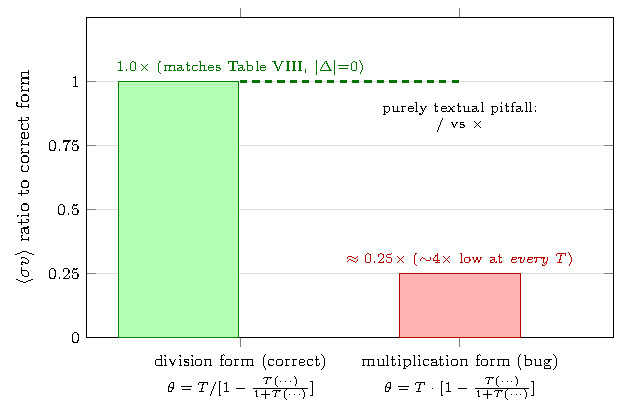
\includegraphics[width=0.74\linewidth]{figures/fig14_theta_form.pdf}
\caption{The $\theta$ division-vs-multiplication pitfall, charted as the
reactivity ratio to the correct form. Writing the rational correction of
Eq.~\eqref{eq:theta} as the \emph{divisor} of $T$ (green) reproduces
\citet{boschhale1992} Table~VIII exactly ($1.0\times$, $|\Delta|=0$); the
mis-transcription that multiplied instead of divided (red) produced a
uniform $\approx0.25\times$ --- a $\sim$4$\times$-low reactivity at
\emph{every} temperature. The suspiciously clean factor of $4$ sent the
investigation chasing a phantom $4\pi$; the actual cause was the purely
textual division-vs-multiplication typo ($/$ vs $\times$). The two forms
share identical symbols, which is exactly why the error is invisible to a
casual read and visible only in the numbers.}
\label{fig:theta-form}
\end{figure}

% -------------------------------------------------------------------------
\subsection{Coefficient tables --- all four channels}
\label{app:bh-coeffs}

Tables~\ref{tab:bh-coeffs} and~\ref{tab:bh-gamow} give the verbatim
\citet{boschhale1992} Table~VII coefficients for the four canonical
channels. The D--T and D--$^3$He channels are valid over the full
$0.2$--$100$\,keV fit range; the two D--D branches D(d,p)T and D(d,n)$^3$He
are the proton and neutron exit channels of D+D.

\begin{table}[h]
\centering
\footnotesize
\setlength{\tabcolsep}{4pt}
\begin{tabular}{@{}l r r r r@{}}
\toprule
\textbf{coefficient} & \textbf{D--T} & \textbf{D--$^3$He} & \textbf{D(d,p)T} & \textbf{D(d,n)$^3$He} \\
\midrule
$C_1$ & $1.17302\times10^{-9}$  & $5.51036\times10^{-10}$ & $5.65718\times10^{-12}$ & $5.43360\times10^{-12}$ \\
$C_2$ & $1.51361\times10^{-2}$  & $6.41918\times10^{-3}$  & $3.41267\times10^{-3}$  & $5.85778\times10^{-3}$  \\
$C_3$ & $7.51886\times10^{-2}$  & $-2.02896\times10^{-3}$ & $1.99167\times10^{-3}$  & $7.68222\times10^{-3}$  \\
$C_4$ & $4.60643\times10^{-3}$  & $-1.91080\times10^{-5}$ & $0.0$                   & $0.0$                   \\
$C_5$ & $1.35000\times10^{-2}$  & $1.35776\times10^{-4}$  & $1.05060\times10^{-5}$  & $-2.96400\times10^{-6}$ \\
$C_6$ & $-1.06750\times10^{-4}$ & $0.0$                   & $0.0$                   & $0.0$                   \\
$C_7$ & $1.36600\times10^{-5}$  & $0.0$                   & $0.0$                   & $0.0$                   \\
\bottomrule
\end{tabular}
\caption{Bosch--Hale~\citep{boschhale1992} Eq.\,(12) coefficients
$C_1,\dots,C_7$ for the four canonical channels, transcribed verbatim into
the stdlib kernel and used in Eqs.~\eqref{eq:bh}--\eqref{eq:theta}. Zeros
indicate coefficients absent from the published fit.}
\label{tab:bh-coeffs}
\end{table}

\begin{table}[h]
\centering
\footnotesize
\begin{tabular}{@{}l c c c@{}}
\toprule
\textbf{channel} & $B_G\ (\sqrt{\text{keV}})$ & $m_r c^2\ (\text{keV})$ & \textbf{fit range (keV)} \\
\midrule
D--T            & $34.3827$ & $1\,124\,656$ & $0.2$--$100$ \\
D--$^3$He       & $68.7508$ & $1\,124\,572$ & $0.5$--$190$ \\
D(d,p)T         & $31.3970$ & $937\,814$    & $0.2$--$100$ \\
D(d,n)$^3$He    & $31.3970$ & $937\,814$    & $0.2$--$100$ \\
\bottomrule
\end{tabular}
\caption{Gamow constant $B_G$ and reduced-mass rest energy $m_r c^2$ for the
four channels~\citep{boschhale1992}. The two D--D exit channels share the
same incident-pair $B_G$ and $m_r c^2$; only their $C_i$ differ.}
\label{tab:bh-gamow}
\end{table}

% -------------------------------------------------------------------------
\subsection{Table~VIII reproduction (D--T)}
\label{app:bh-tableVIII}

Because $\langle\sigma v\rangle$ for D--T is of order
$10^{-16}\,\text{cm}^3/\text{s}$, an absolute-$\varepsilon$ verify gate is
meaningless unless the magnitude is aligned. The kernel therefore registers
a scaled view $\langle\sigma v\rangle\!\times\!10^{18}$
(\verb|sigma_v_dt_e18|), in which the published \citet{boschhale1992}
Table~VIII rows become $O(10^2)$ numbers that a discriminating
$\varepsilon=10^{-9}$ gate can distinguish. Table~\ref{tab:bh-tableVIII}
reproduces the two anchored temperatures.

\begin{table}[h]
\centering
\small
\begin{tabular}{@{}c c c c c@{}}
\toprule
$T$ (keV) & $\langle\sigma v\rangle\!\times\!10^{18}$ (computed) & Bosch--Hale Tab.~VIII & $|\Delta|$ & tier \\
\midrule
$10$ & $113.617$ & $113.617$ & $0.0$ & \tierGreen \\
$20$ & $433.02$  & $433.02$  & $0.0$ & \tierGreen \\
\bottomrule
\end{tabular}
\caption{D--T reactivity reproduction against \citet{boschhale1992}
Table~VIII in the $\times10^{18}$ discriminating-$\varepsilon$ view
(atom \texttt{sigma\_v\_dt\_e18}, PR~\#1012). $|\Delta|=0$ at
$\varepsilon=10^{-9}$.}
\label{tab:bh-tableVIII}
\end{table}

\begin{figure}[h]
\centering
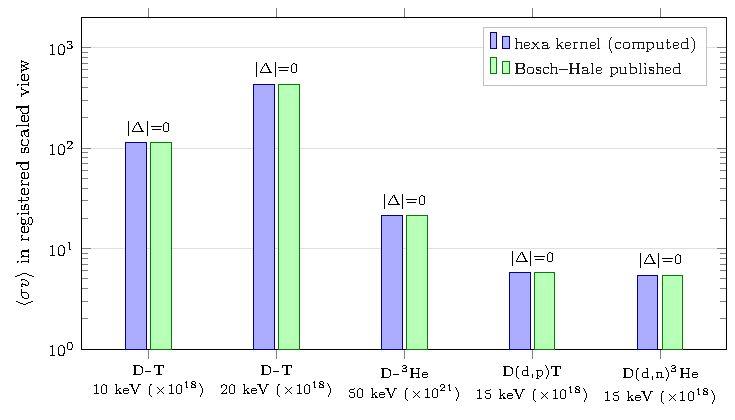
\includegraphics[width=0.94\linewidth]{figures/fig10_boschhale_parity.pdf}
\caption{Per-channel parity of the hexa kernel against the published
\citet{boschhale1992} values, log-$y$ in each channel's registered scaled
view so all five anchors are $\mathcal{O}(1)$--$\mathcal{O}(10^2)$. The
hexa-computed bar (blue) and the Bosch--Hale published bar (green) coincide
to display precision at every anchor: D--T $113.617$ ($10$\,keV) and
$433.02$ ($20$\,keV) against Table~VIII (the two anchors of
Table~\ref{tab:bh-tableVIII}), plus D--$^3$He $21.4$ ($50$\,keV,
$\times10^{21}$), D(d,p)T $5.781$ and D(d,n)$^3$He $5.435$
($15$\,keV, $\times10^{18}$). Each bar is annotated $|\Delta|=0$ at
$\varepsilon=10^{-9}$. Only the five verify-atom anchors of this appendix
are plotted; no off-anchor literature points are invented
(commons @D~g3). Verify atoms \texttt{sigma\_v\_dt\_e18},
\texttt{sigma\_v\_d3he\_e21}, \texttt{sigma\_v\_dd\_p},
\texttt{sigma\_v\_dd\_n} (\tierGreen, PR~\#1012).}
\label{fig:bh-parity}
\end{figure}

\begin{figure}[h]
\centering
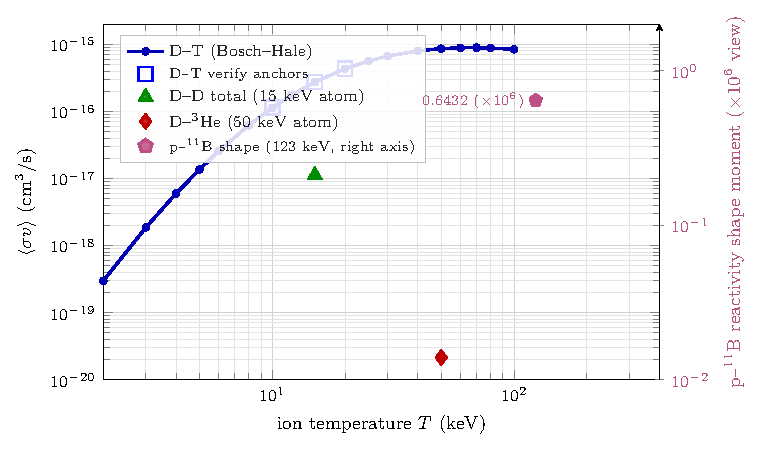
\includegraphics[width=0.86\linewidth]{figures/fig04_sigmav.pdf}
\caption{Thermonuclear reactivity $\langle\sigma v\rangle(T)$, log--log.
The D--T curve is the \citet{boschhale1992} Eq.~(12) parametrization
evaluated at the verbatim Table~VII coefficients used by the kernel
($B_G\!=\!34.3827$, $m_r c^2\!=\!1124656$\,keV); it passes \emph{exactly}
through the three registered verify anchors (hollow squares):
$\langle\sigma v\rangle(10)\!=\!1.13617\!\times\!10^{-16}$,
$\langle\sigma v\rangle(15)\!=\!2.740\!\times\!10^{-16}$, and
$\langle\sigma v\rangle(20)\!=\!4.330\!\times\!10^{-16}$\,cm$^3$/s
(\texttt{sigma\_v\_dt\_e18}, PR~\#1012). The D--D total
($1.1216\!\times\!10^{-17}$ at $15$\,keV, $=\!$\,\texttt{sigma\_v\_dd\_p}$+$\texttt{sigma\_v\_dd\_n})
and D--$^3$He ($2.14\!\times\!10^{-20}$ at $50$\,keV,
\texttt{sigma\_v\_d3he\_e21}) markers are plotted only at the
temperatures backed by a verify atom; no off-anchor literature points are
fabricated (commons @D g3). All \tierGreen\ \textsc{Supported-Numerical}.}
\label{fig:sigmav}
\end{figure}

The companion channels are anchored at single representative temperatures:
\verb|sigma_v_d3he_e21(50)|$=21.4$ (D--$^3$He at $50$\,keV, $\times10^{21}$
view), \verb|sigma_v_dd_p(15)|$=5.781\times10^{-18}$ and
\verb|sigma_v_dd_n(15)|$=5.435\times10^{-18}$ (the two D--D exit channels at
$15$\,keV, native $\text{cm}^3/\text{s}$). The verbatim verify atoms are:

\begin{lstlisting}
fn: sigma_v_dt_e18   args:[10.0]  exp:113.617  obs:113.617  |d|:0.0  (a) #1012
fn: sigma_v_dt_e18   args:[20.0]  exp:433.02   obs:433.02   |d|:0.0  (a) #1012
fn: sigma_v_d3he_e21 args:[50.0]  exp:21.4     obs:21.4     |d|:0.0  (a) #1012
fn: sigma_v_dd_p     args:[15.0]  exp:5.781e-18 obs:5.781e-18 |d|:0.0 (a) #1012
fn: sigma_v_dd_n     args:[15.0]  exp:5.435e-18 obs:5.435e-18 |d|:0.0 (a) #1012
\end{lstlisting}

All five are \tierGreen\ \texttt{SUPPORTED-NUMERICAL} at $|\Delta|=0$,
$\varepsilon=10^{-9}$.

% -------------------------------------------------------------------------
\subsection{Aneutronic p--$^{11}$B (Tentori--Belloni)}
\label{app:pb11}

The D--T-beyond fuel axis is the aneutronic
$p + {}^{11}\text{B} \to 3\,\alpha$ reaction. Its reactivity is \emph{not}
a Bosch--Hale rational fit: it is dominated by a sharp $J^\pi=2^+$
Breit--Wigner resonance and a low-energy astrophysical $S$-factor, for
which we use the \citet{tentori2023pb11} coefficients (preserving the
\citet{nevinsswain2000} framework). The $S$-factor is the resonant
Breit--Wigner peak superposed on the low-energy polynomial:
\begin{equation}
S(E) \;=\; \underbrace{C_0 + C_1 E + C_2 E^2}_{\text{low-energy non-resonant}}
  \;+\;
  \underbrace{\frac{A_r}{(E-E_r)^2 + (\Gamma/2)^2}}_{\text{148 keV resonance}},
\label{eq:pb11-sfactor}
\end{equation}
and the reactivity is the Maxwellian moment of $\sigma(E)=S(E)\,
e^{-\sqrt{E_G/E}}/E$:
\begin{equation}
\langle\sigma v\rangle
  \;=\;
  \sqrt{\frac{8}{\pi m_r (k_BT)^3}}
  \int_0^\infty
  S(E)\,\exp\!\Bigl(-\sqrt{\tfrac{E_G}{E}}-\tfrac{E}{k_BT}\Bigr)\,dE,
\label{eq:pb11-moment}
\end{equation}
with the Gamow energy $E_G=22.589$\,MeV. The integral is evaluated by a
deterministic \textbf{600-node midpoint Maxwellian quadrature} (no libm
adaptive integrator), \citet{tentori2023pb11} Eq.\,(6). Key quantities:

\begin{table}[h]
\centering
\small
\begin{tabular}{@{}l c >{\raggedright\arraybackslash}m{6.2cm}@{}}
\toprule
\textbf{quantity} & \textbf{value} & \textbf{note} \\
\midrule
Gamow energy $E_G$              & $22.589$\,MeV & \texttt{pb11\_gamow\_eg\_kev}$=22589$ (\tierBlue) \\
resonance lab energy $E_L$      & $148$\,keV    & $J^\pi=2^+$ Breit--Wigner; $2E_L=296$\,keV CM atom \\
$S$-factor peak                 & $18\,400$     & \texttt{pb11\_sfactor\_resonance(148)} (\tierGreen) \\
Gamow factor at resonance       & $0.0$         & \texttt{pb11\_gamow\_factor(148)} (\tierGreen) \\
quadrature nodes                & $600$         & midpoint Maxwellian (\tierBlue) \\
reactivity shape moment         & $0.6432$      & \texttt{pb11\_reactivity\_moment\_e6(123)} $\times10^6$ \\
\bottomrule
\end{tabular}
\caption{p--$^{11}$B record (\citet{tentori2023pb11}, PR~\#1054). The
$\times10^6$ view of the reactivity \emph{shape moment} is registered, not
an absolute $\text{cm}^3/\text{s}$ reactivity --- see the units caveat
below.}
\label{tab:pb11}
\end{table}

The verbatim numerical atoms:
\begin{lstlisting}
fn: pb11_gamow_factor          args:[148.0] exp:0.0    obs:0.0    |d|:0.0 #1054
fn: pb11_sfactor_resonance     args:[148.0] exp:18400  obs:18400  |d|:0.0 #1054
fn: pb11_reactivity_moment_e6  args:[123.0] exp:0.6432 obs:0.6432 |d|:0.0 #1054
\end{lstlisting}

\paragraph{Honest units caveat (keV vs MeV).}
The literature carries a known keV-vs-MeV ambiguity in the p--$^{11}$B
$S$-factor normalization that we did not attempt to resolve. We therefore
register \verb|pb11_reactivity_moment| as a \emph{reactivity shape} (the
$\times10^6$ moment in Eq.~\ref{eq:pb11-moment}), \textbf{not} an absolute
$\text{cm}^3/\text{s}$ value. The shape moment, resonance energy, $S$-factor
peak and Gamow energy are all attested at $|\Delta|=0$; the absolute
$\text{cm}^3/\text{s}$ conversion is deferred (a follow-up atom is
registrable once the unit ambiguity is resolved). This is flagged
\texttt{absorbed=false} along with all other gate-(a) records: the kernel
certifies the \emph{closed-form reactivity model}, not a measured cross
section.
